\documentclass[10pt]{article}

\usepackage[letterpaper,margin=0.78in]{geometry}
\usepackage[T1]{fontenc}
\usepackage{lmodern}
\usepackage{microtype}
\usepackage{graphicx}
\usepackage{booktabs}
\usepackage{array}
\usepackage{caption}
\usepackage{subcaption}
\usepackage{amsmath}
\usepackage[numbers,sort&compress]{natbib}
\usepackage[colorlinks=true,linkcolor=blue,citecolor=blue,urlcolor=blue]{hyperref}

\setlength{\parindent}{0pt}
\setlength{\parskip}{4pt}
\setlength{\textfloatsep}{8pt plus 2pt minus 2pt}
\setlength{\floatsep}{8pt plus 2pt minus 2pt}
\setlength{\intextsep}{8pt plus 2pt minus 2pt}
\captionsetup{font=small,labelfont=bf}

\newcommand{\pd}{prefill--decode}
\newcommand{\pdratio}{PD/baseline}
\newcommand{\ttft}{TTFT}
\newcommand{\tbt}{TBT}
\newcommand{\etoe}{E2E}

\title{\vspace{-0.35in}When Does Prefill--Decode Disaggregation Help?\\
\large A Parametric Study of Trade-offs in LLM Serving}
\author{Course Project Report}
\date{}

\begin{document}
\maketitle
\vspace{-0.25in}

\begin{abstract}
Large language model (LLM) serving systems split each request into a prompt or prefill phase, which processes the input context, and an autoregressive decode phase, which emits output tokens. Recent systems argue that these two phases have different resource characteristics and should be scheduled on separate resources. This project asks a narrower empirical question: under what workload and resource conditions does \pd{} disaggregation actually reduce tail latency? Using SplitwiseSim, we compare a coupled baseline against \pd{} disaggregation across prompt length, output length, request rate, KV-cache transfer bandwidth, and prompt:decode resource split. Across a 144-point A100-only main sweep, \pd{} improves p99 time-between-tokens in 109/144 cases and p99 end-to-end latency in 90/144 cases, but improves standard p99 time-to-first-token in only 17/144 cases. A focused split sweep shows that resource allocation is first-order: at 25 GB/s KV bandwidth, a 6:2 prompt:decode split wins all 27 moderate-workload E2E comparisons, while a 2:6 split wins only 18/27. We also introduce prompt spillover as a diagnostic for Splitwise-style elastic scheduling; when prompt work spills onto token-side instances, the E2E advantage often collapses. Overall, \pd{} is not a universal win. It helps when decode-side isolation and batching outweigh prompt-side queueing and KV handoff cost, and hurts when the configured split under-provisions the bottleneck phase.
\end{abstract}

\section{Introduction}
Serving generative LLMs is increasingly a systems problem as much as a modeling problem. An inference request has two phases with very different behavior. The prefill phase consumes the prompt in parallel and is relatively compute intensive; the decode phase generates one token at a time and is often memory-bandwidth dominated. This asymmetry motivates systems such as Splitwise~\citep{splitwise2024}, DistServe~\citep{distserve2024}, and TetriInfer~\citep{tetriinfer2024}, which separate or partially separate prefill and decode work so each phase can be provisioned and scheduled differently.

The idea is appealing, but it is not free. A disaggregated request must move its KV cache from the prefill side to the decode side, and a fixed resource split can create a new bottleneck. If the prompt side is under-provisioned, requests may wait before the first token. If the decode side is under-provisioned, output tokens become slow or bursty. If KV transfer is slow, the handoff path can dominate even when each individual phase is efficient. This creates a practical question that is not answered by saying that prefill and decode are ``different'': when does separating them help, and when does it hurt?

This report presents a simulator-based parametric study using SplitwiseSim, a discrete-event simulator released with the Splitwise project. The study compares a coupled baseline, where all instances serve both phases, against \pd{} configurations. We focus on tail-latency metrics used in LLM serving: time to first token (TTFT), time between tokens (TBT), and end-to-end request latency (E2E). We report \pdratio{} values, where a ratio below 1.0 means disaggregation is faster than the coupled baseline.

\textbf{Key findings.} First, \pd{} most reliably improves decode-side behavior. In the main 144-point sweep, p99 TBT improves in 75.7\% of cases, while p99 E2E improves in 62.5\%. Second, standard TTFT is much harder to improve: it improves in only 11.8\% of the main sweep, because prompt-side queueing can dominate first-token latency. Third, resource split is a first-order parameter. In the focused 81-case split sweep, the prefill-heavy 6:2 split has the best median E2E ratio and wins every split-specific E2E comparison, while the decode-heavy 2:6 split often fails. Fourth, elastic borrowing in Splitwise-style MixedPool is not a bug; it is a useful behavior, but prompt spillover onto token-side instances is a strong diagnostic that the configured split no longer preserves decode isolation.

The practical takeaway is conditional rather than absolute: \pd{} helps inside a capacity-balanced region. A system designer should not evaluate \pd{} only as an architectural switch, but as a joint choice of workload shape, arrival rate, network bandwidth, and prompt/decode resource allocation.

\section{Background and Related Work}
\textbf{LLM serving phases.} Autoregressive transformer inference naturally separates into prefill and decode. The prefill phase processes all input tokens and constructs KV state. The decode phase repeatedly consumes the current KV state and emits the next token. Prior serving systems such as Orca and vLLM improve batching, iteration-level scheduling, and KV-cache memory management for generative inference~\citep{orca2022,vllm2023}. These systems reduce waste in coupled serving, but prefill and decode can still interfere because they share the same accelerators and batching decisions.

\textbf{Disaggregation.} Splitwise argues that prompt computation and token generation have different compute, memory, latency, and power characteristics, and proposes phase splitting across separate machines~\citep{splitwise2024}. DistServe similarly assigns prefill and decoding to different GPUs, and co-optimizes resource allocation and parallelism under TTFT and TPOT requirements~\citep{distserve2024}. TetriInfer studies mixed downstream workloads and uses disaggregation plus workload-aware scheduling to reduce interference~\citep{tetriinfer2024}. These systems support the motivation for this project: \pd{} is promising, but resource allocation and workload shape determine whether the promise materializes.

\textbf{This study's scope.} The goal here is not to reproduce a full production system. Instead, we use SplitwiseSim to run many low-cost CPU simulations and map the qualitative boundary where disaggregation helps or hurts. This makes the study complementary to implementation papers: we can sweep many prompt lengths, output lengths, rates, bandwidths, and splits quickly, but the conclusions should be read as simulator-level evidence rather than direct GPU measurements.

\section{Methodology}
\subsection{Simulator and Systems Compared}
Experiments use SplitwiseSim, the simulator associated with Splitwise. The base model is Llama-2-70B~\citep{llama2}, using SplitwiseSim's database performance model. All main experiments use A100-only instances so that the study isolates phase separation and resource allocation rather than heterogeneous hardware choice.

We compare two primary systems:
\begin{itemize}
  \item \textbf{Coupled baseline}: all 8 A100 instances serve both prefill and decode using the \texttt{token\_jsq} scheduler.
  \item \textbf{PD-MixedPool}: instances are initially divided into prompt-side and token-side pools, but idle capacity can be borrowed elastically across pools. This models the Splitwise-style MixedPool behavior in the simulator.
\end{itemize}

We also use a strict no-borrow \pd{} control, where prompt work can run only on prompt instances and decode work only on token instances. The strict control is not the main system; it is a diagnostic that clarifies whether a result comes from true phase separation or from MixedPool borrowing.

\subsection{Workloads and Variables}
The main sweep contains 144 complete PD/baseline pairs:
\[
4 \text{ prompts} \times 3 \text{ outputs} \times 3 \text{ rates} \times 4 \text{ bandwidths}=144.
\]
Prompt lengths are 128, 512, 1024, and 2048 tokens; output lengths are 16, 64, and 256 tokens; request rates are 20, 50, and 100 requests/s; and KV bandwidths are 50, 25, 12.5, and 3.125 GB/s. The main \pd{} split is 4:4 prompt:decode.

Follow-up experiments refine the boundary. A focused split sweep fixes bandwidth at 25 GB/s and evaluates prompt lengths 128, 256, and 512, output lengths 64, 128, and 256, rates 20, 50, and 100 requests/s, and splits 2:6, 4:4, and 6:2. This produces 27 baseline runs and 81 \pd{} runs. An overlap variant approximates hiding most KV transfer cost by using 10x effective KV bandwidth, following the existing overlap scheduler convention in SplitwiseSim. Finally, a strict no-borrow sweep evaluates prompt lengths up to 1024 with the same 8-instance budget.

\begin{table}[t]
\centering
\small
\caption{Main experimental setup.}
\label{tab:setup}
\begin{tabular}{ll}
\toprule
Component & Setting \\
\midrule
Model & Llama-2-70B \\
Hardware & A100-only simulator instances \\
Total instances & 8 \\
Main baseline & Coupled \texttt{token\_jsq} \\
Main PD scheduler & MixedPool with 4:4 prompt:decode split \\
Arrival process & Synthetic Poisson traces \\
Trace duration & 10 seconds, with selected 30-second checks \\
Main variables & Prompt length, output length, request rate, KV bandwidth \\
Focused variables & Prompt:decode split, overlap, strict no-borrow control \\
\bottomrule
\end{tabular}
\end{table}

\subsection{Metrics}
All primary results use p99 tail latency. TTFT measures time to first token as recorded by SplitwiseSim. In this simulator, the prompt task processes the prompt and generates the first output token; KV transfer happens after this point before the remaining decode tokens continue. TBT measures time between output tokens and therefore captures decode smoothness. E2E measures total request latency from arrival to completion.

We also report a diagnostic metric:
\[
\text{handoff-adjusted TTFT} = \text{TTFT} + \text{nth-token overhead}.
\]
Older CSVs in this repository call it \texttt{effective\_ttft}. In this report, we call it handoff-adjusted TTFT because it is not the standard user-visible TTFT. It captures KV transfer and token-side queueing before decode continuation, so it is useful for diagnosing the handoff penalty introduced by \pd{}.

\section{Results}
\subsection{PD Improves Decode Latency More Reliably Than TTFT}
Table~\ref{tab:main-summary} summarizes the 144-point main sweep. The clearest result is metric-specific: \pd{} helps TBT much more reliably than TTFT. TBT improves in 109/144 cases with a median ratio of 0.941. E2E improves in 90/144 cases with a median ratio of 0.962. In contrast, standard TTFT improves in only 17/144 cases, and handoff-adjusted TTFT improves in only 8/144.

\begin{table}[t]
\centering
\small
\caption{Main 144-point sweep. Ratios are PD/baseline; values below 1.0 mean PD is faster.}
\label{tab:main-summary}
\begin{tabular}{lrrr}
\toprule
Metric & PD better & Share & Median ratio \\
\midrule
TTFT p99 & 17/144 & 11.8\% & 1.190 \\
Handoff-adjusted TTFT p99 & 8/144 & 5.6\% & 1.675 \\
TBT p99 & 109/144 & 75.7\% & 0.941 \\
E2E p99 & 90/144 & 62.5\% & 0.962 \\
\bottomrule
\end{tabular}
\end{table}

\begin{figure}[t]
\centering
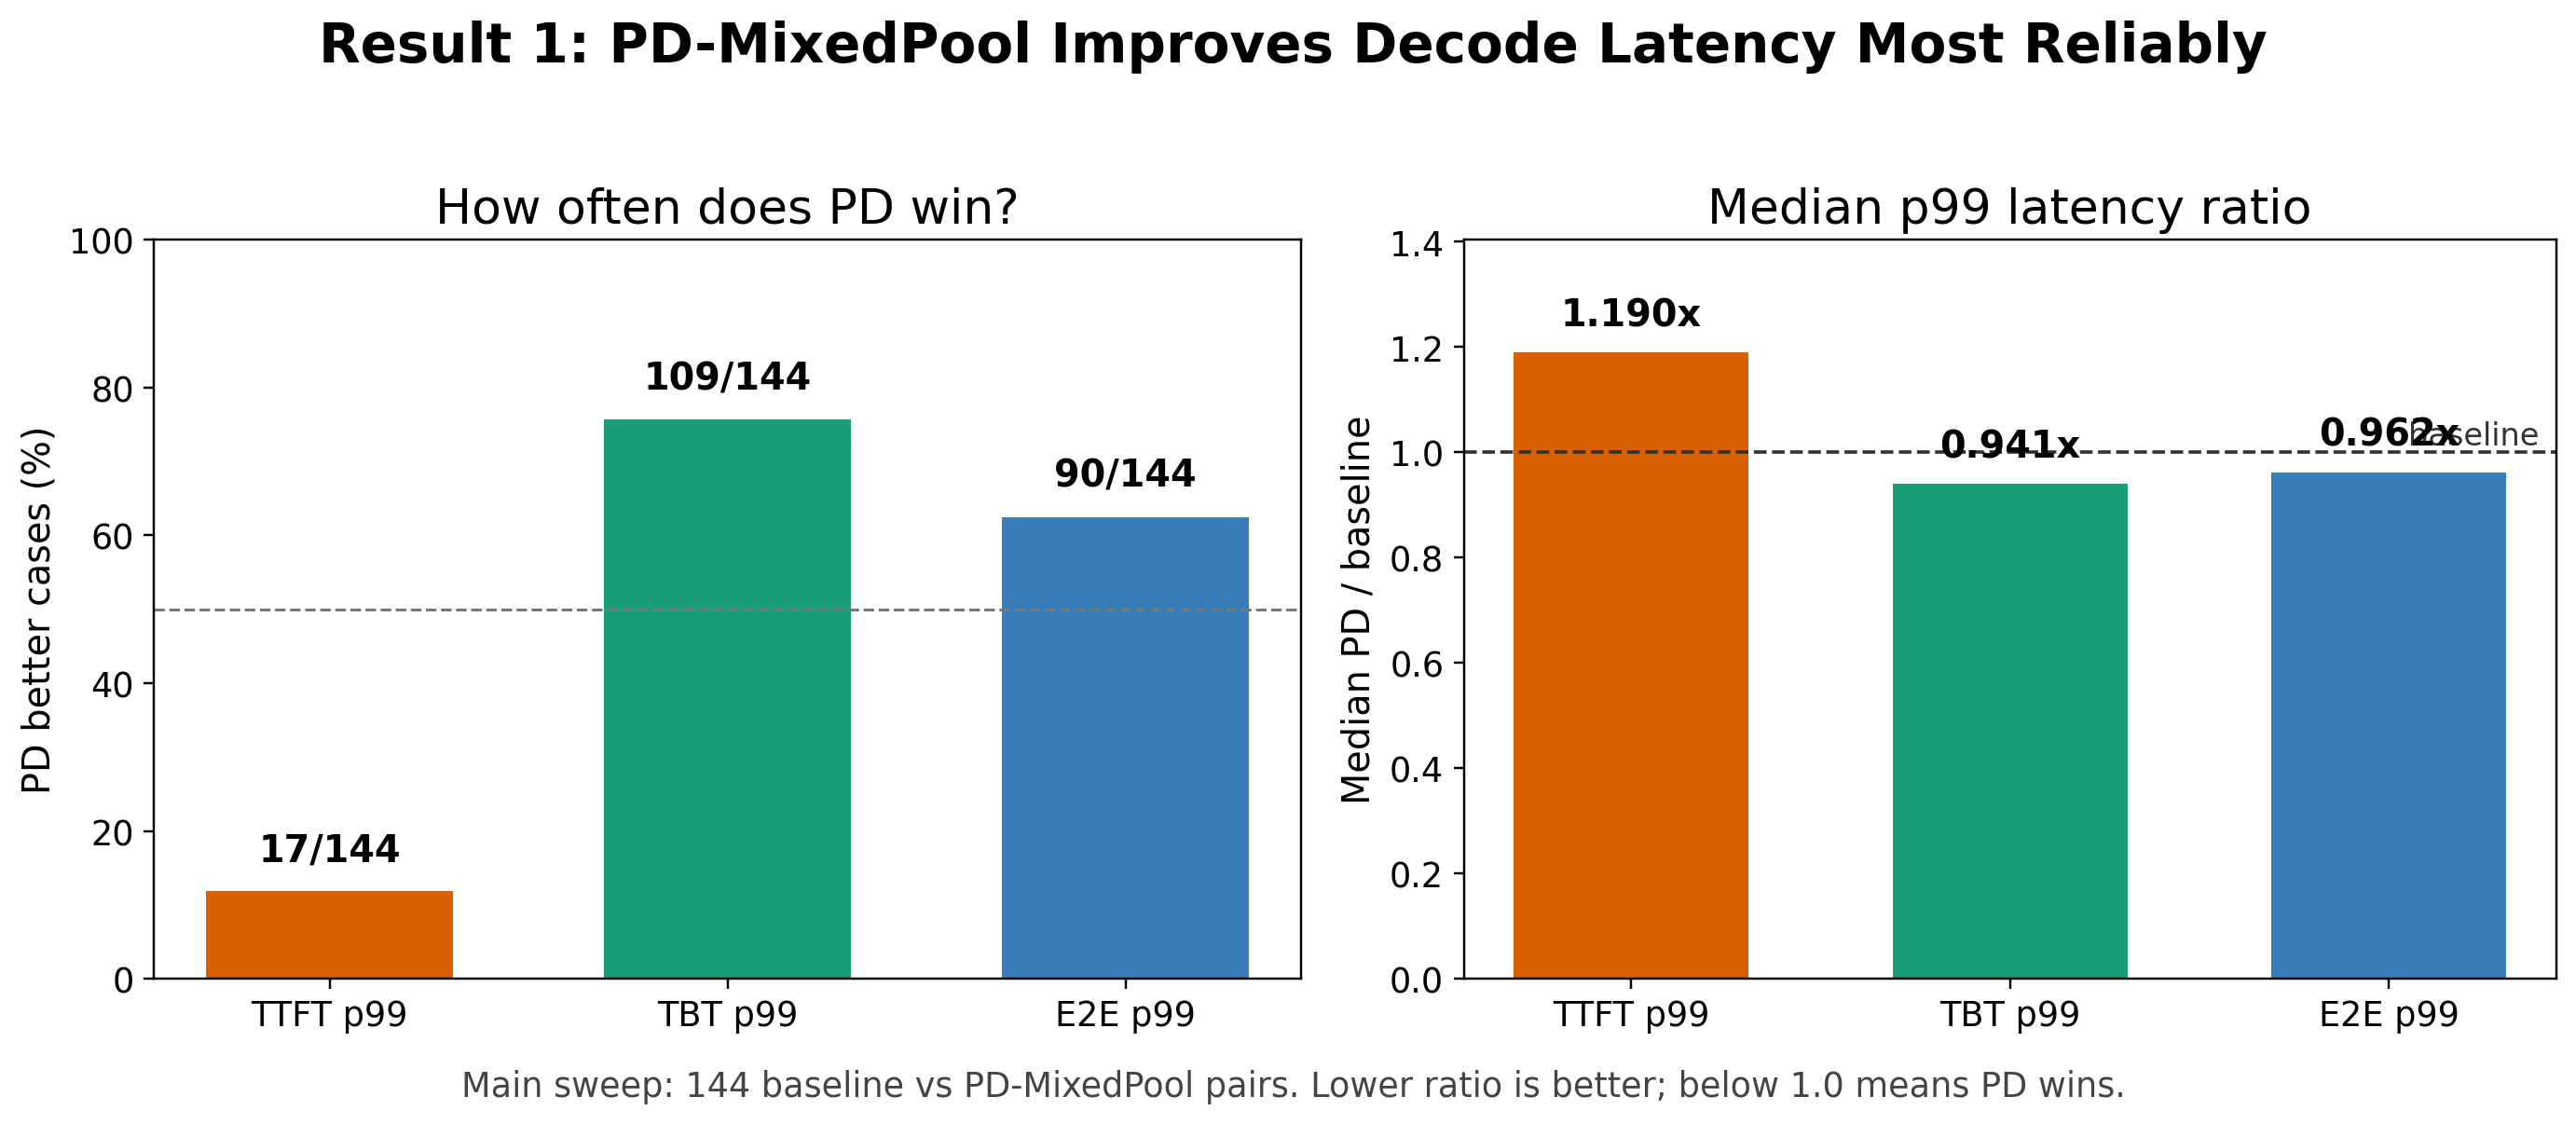
\includegraphics[width=0.92\linewidth]{figures/metric_overview.png}
\caption{Metric-level trade-off for the main study. Green points indicate PD wins; red points indicate PD losses. PD most reliably improves TBT and often improves E2E, while TTFT is harder to improve.}
\label{fig:metric-overview}
\end{figure}

This is consistent with the architecture. Disaggregation isolates decode from large prefill batches, which can smooth token generation. But it does not automatically reduce first-token latency: the prompt side can queue, and after the first token the request still has to hand off KV state to the decode side. The best observed E2E case occurs at prompt=128, output=64, rate=100 requests/s, bandwidth=50 GB/s, where \pd{} reaches an E2E ratio of 0.671. The worst observed E2E case occurs at prompt=2048, output=256, rate=100 requests/s, bandwidth=12.5 GB/s, where the E2E ratio is 1.942. The same favorable and unfavorable regimes hold across three independent arrival traces at 25 GB/s, with mean E2E ratios of 0.664 and 1.729 respectively.

\subsection{Resource Split Is a First-Order Parameter}
The focused split sweep asks whether a fixed 4:4 split is a good default. The answer is no. In the 81-case split matrix at 25 GB/s, 6:2 has the best median E2E ratio and wins every split-specific comparison; 4:4 is also strong; 2:6 is fragile. Table~\ref{tab:split-summary} shows the split-level summary.

\begin{table}[t]
\centering
\small
\caption{Focused resource-split sweep over 81 PD runs at 25 GB/s.}
\label{tab:split-summary}
\begin{tabular}{lrrrr}
\toprule
Prompt:decode split & E2E wins & Median E2E & Median TTFT & Median TBT \\
\midrule
2:6 & 18/27 & 0.937 & 2.550 & 0.929 \\
4:4 & 25/27 & 0.852 & 1.133 & 0.843 \\
6:2 & 27/27 & 0.828 & 0.956 & 0.825 \\
\bottomrule
\end{tabular}
\end{table}

\begin{figure}[t]
\centering
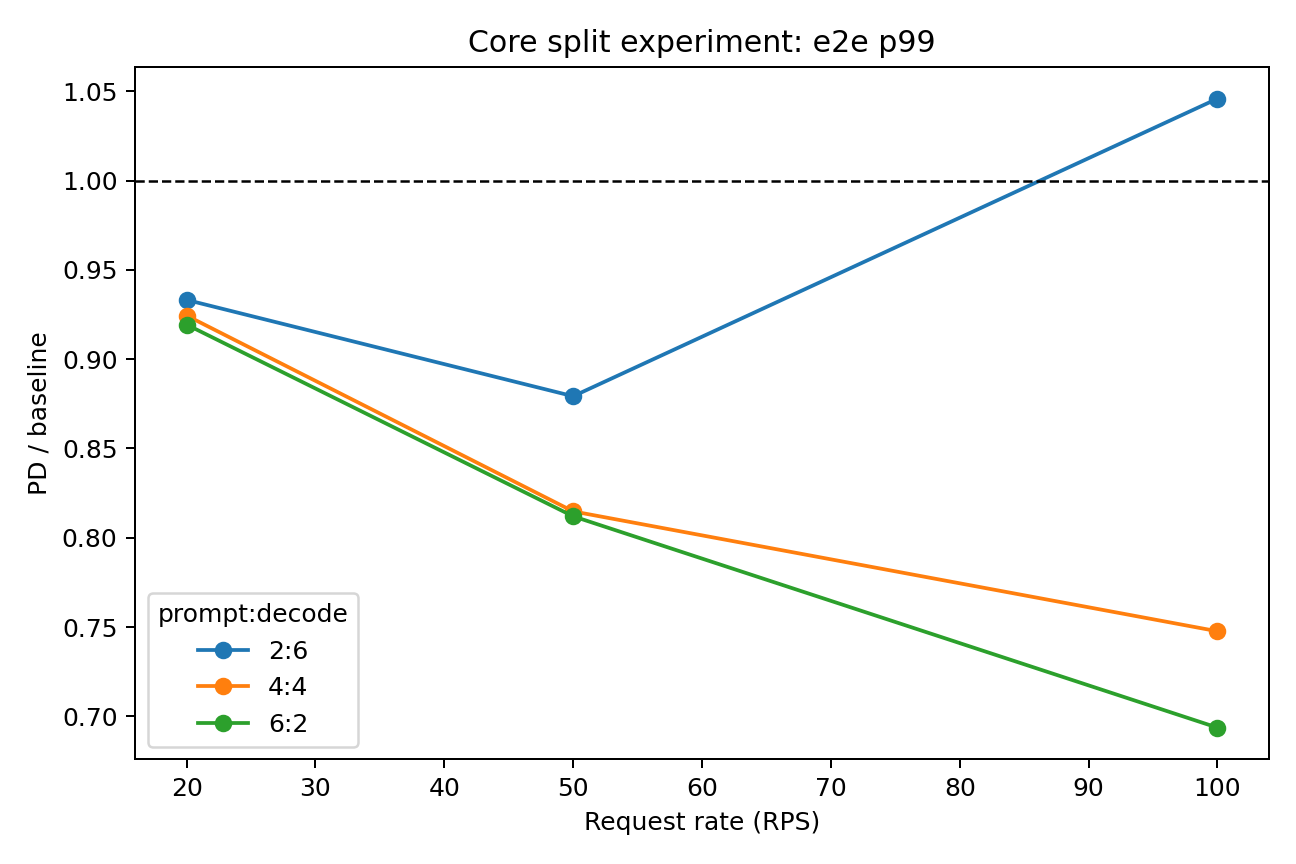
\includegraphics[width=0.82\linewidth]{figures/e2e_by_rate.png}
\caption{E2E p99 ratio by request rate and prompt:decode split in the focused split sweep. The prefill-heavy 6:2 split becomes more favorable as rate increases, while the decode-heavy 2:6 split crosses above 1.0 at high rate.}
\label{fig:rate-split}
\end{figure}

The result may look counterintuitive if one expects higher rate or longer outputs to always favor more decode instances. In this simulator setup, prompt work is frequently the limiting phase for prompt lengths up to 512. Giving only two instances to prefill creates large prompt queues, so a decode-heavy 2:6 split can lose even when TBT improves. Figure~\ref{fig:rate-split} makes this boundary visible: as request rate increases, the wrong split becomes increasingly costly. This supports the DistServe-style argument that \pd{} requires phase-aware resource allocation, not merely phase separation.

\subsection{Overlap Helps Handoff, But Does Not Remove Split Sensitivity}
The overlap experiment repeats the focused split sweep with an overlap scheduler that approximates hiding much of the KV transfer cost. Overlap improves handoff-adjusted TTFT from a median ratio of 1.555 to 1.440 and slightly improves TBT from 0.853 to 0.845. However, the median E2E ratio remains 0.869, and the best-split distribution is unchanged: 6:2 is best for 17/27 workload points, 4:4 for 9/27, and 2:6 for 1/27.

This suggests that network and handoff optimization matter, but bandwidth alone does not explain the full boundary. Once KV transfer is partly hidden, prompt/decode capacity balance remains the dominant question. Put another way, making the bridge faster does not help if too many cars are waiting before the bridge.

\subsection{Prompt Spillover Diagnoses When Elastic PD Stops Being Isolated}
MixedPool can borrow idle capacity across prompt and token pools. This behavior is intentional and can improve utilization, but it also means that ``PD'' is not always strictly separated. To diagnose this, we compute prompt spillover: the fraction of prompt work that runs on instances originally allocated to the token side. In the core overlap sweep, no-spillover cases are clean wins: 66/66 cases improve E2E, with median E2E ratio 0.837. When prompt spillover exceeds 10\%, only 2/12 cases improve E2E.

\begin{figure}[t]
\centering
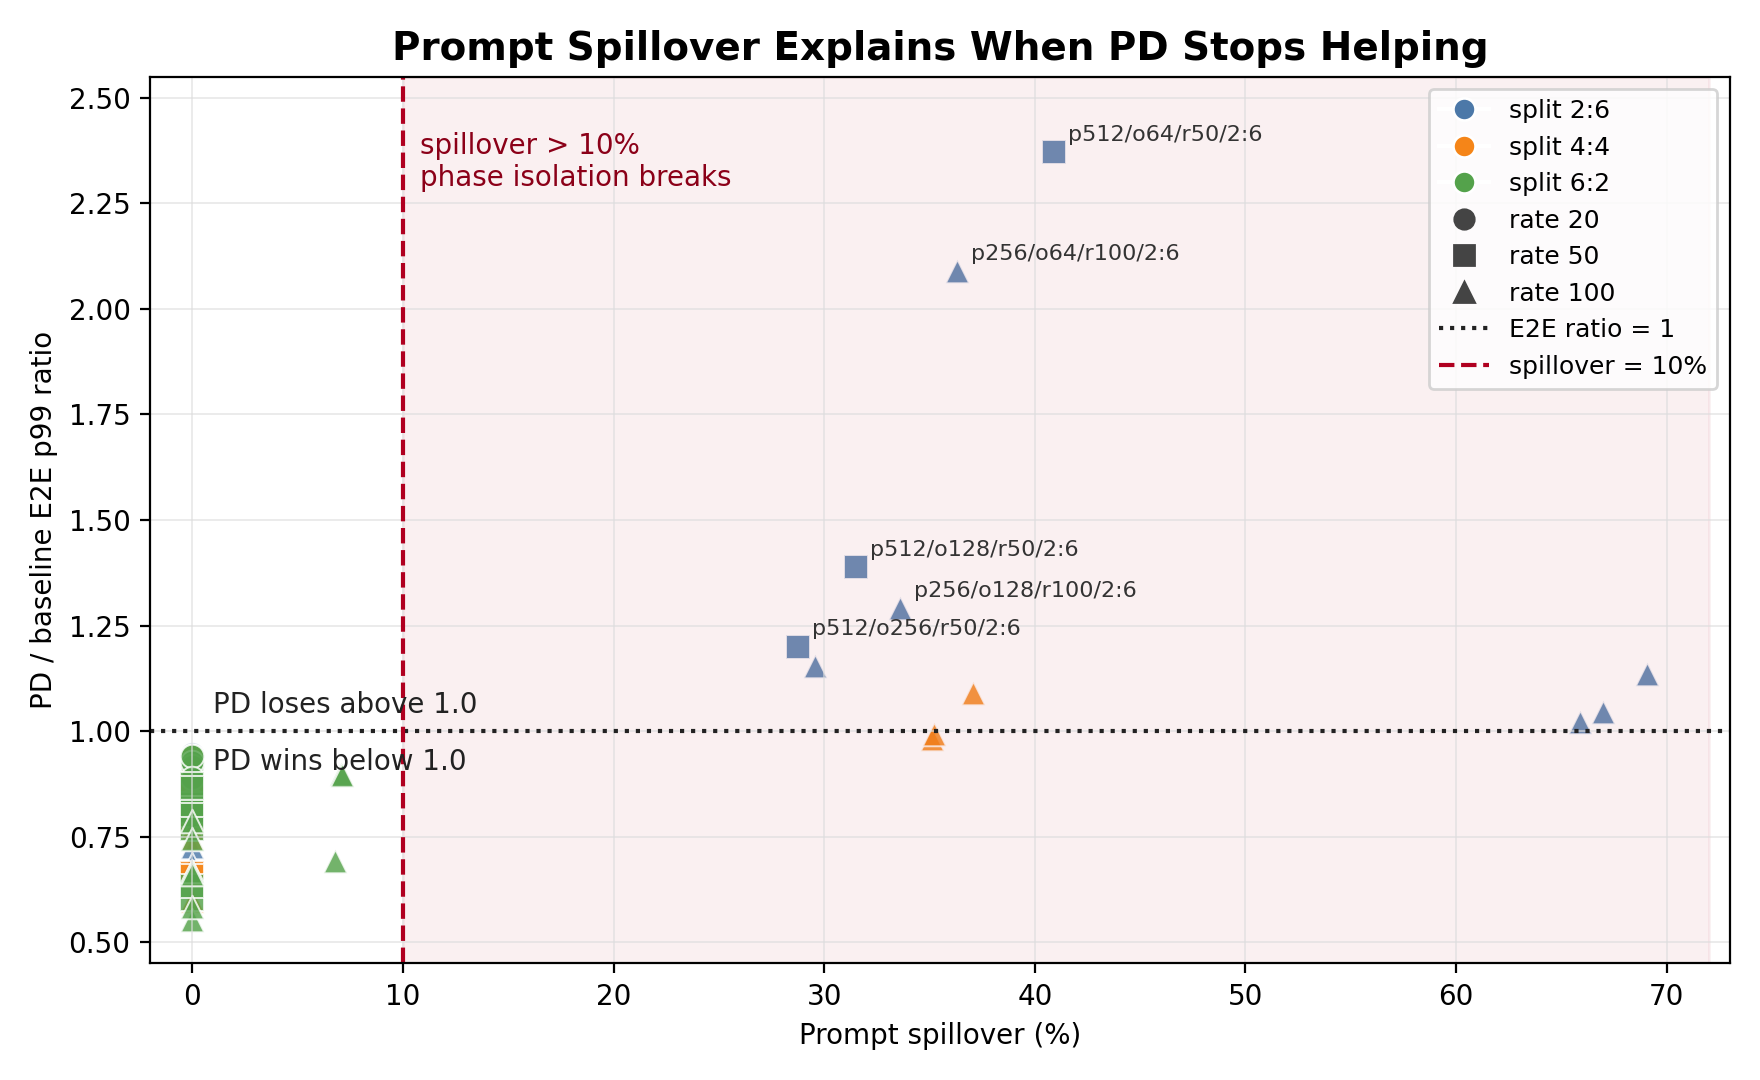
\includegraphics[width=0.94\linewidth]{figures/prompt_spillover_boundary.png}
\caption{Prompt spillover boundary in the core overlap sweep. Each cell reports spillover percentage and E2E ratio. Spillover is a MixedPool-specific diagnostic: it indicates that the configured split can no longer preserve phase isolation.}
\label{fig:spillover}
\end{figure}

Spillover should not be interpreted as a universal overload metric. It is a scheduler-specific signal: in this repository, instances are created with prompt-side IDs first and token-side IDs second, and request traces record the runner instance for each task. If prompt work appears on token-side instances, the MixedPool scheduler has borrowed capacity. This does not prove that the entire system is globally overloaded, but it does show that the configured prompt/decode split is failing to preserve the intended separation. In our data, that is exactly where E2E wins become unreliable.

\subsection{Strict No-Borrow Control Clarifies the Boundary}
The strict no-borrow control removes elastic borrowing and asks what happens when phase separation is enforced. Across 108 strict cases, \pd{} improves TBT in 103/108 cases and E2E in 75/108 cases, but improves TTFT in only 22/108. The split-level boundary becomes sharper: the 2:6 split has median E2E ratio 1.019 and median TTFT ratio 6.638, while 6:2 has median E2E ratio 0.823 and median TTFT ratio 1.034.

\begin{table}[t]
\centering
\small
\caption{Strict no-borrow control. Enforcing separation makes bad splits more visible.}
\label{tab:strict-summary}
\begin{tabular}{lrrrr}
\toprule
Prompt:decode split & E2E wins & Median E2E & Median TTFT & Median handoff TTFT \\
\midrule
2:6 & 18/36 & 1.019 & 6.638 & 5.545 \\
4:4 & 27/36 & 0.873 & 1.377 & 1.595 \\
6:2 & 30/36 & 0.823 & 1.034 & 1.239 \\
\bottomrule
\end{tabular}
\end{table}

Prompt length also exposes the boundary. Strict \pd{} wins E2E in 27/27 cases at prompt length 128, 23/27 at 256, 17/27 at 512, and only 8/27 at 1024. This pattern is important for the report's main claim. Longer prompts do create more opportunity for phase specialization, but only if the prompt side has enough capacity. If prompt demand grows faster than prompt capacity, disaggregation amplifies the bottleneck instead of removing it.

\section{Discussion}
\textbf{Why does TTFT often get worse?} In SplitwiseSim, TTFT is recorded when the prompt task finishes and the first output token is produced. \pd{} can still make TTFT worse because the prompt-side pool is smaller than the coupled baseline's shared pool. In a 4:4 split, only four instances are primarily available for prefill, while the baseline has eight coupled instances that can all process prompt work. If arrivals are high or prompts are long, prompt-side queueing can offset any phase-specialization benefit.

\textbf{Why can E2E improve while TTFT worsens?} E2E includes the entire generation. For longer outputs or higher rates, decode smoothness can dominate total tail latency. \pd{} may delay the first token but reduce per-token delay enough to lower E2E. This is why TBT is the most reliable win in the experiments and why E2E improves more often than TTFT.

\textbf{Why is bandwidth not the only answer?} KV bandwidth affects the handoff path, and overlap reduces handoff-adjusted TTFT. But many E2E outcomes are governed by queueing and split balance. If the prompt side is under-provisioned, increasing bandwidth does not remove the prompt queue. If the decode side is under-provisioned, prefill capacity alone does not smooth generation. The bandwidth result is therefore not contradictory: KV transfer is one cost, but not the only bottleneck.

\textbf{Relation to prior work.} The results align with the spirit of Splitwise and DistServe rather than contradicting them. Prior work argues that the phases should be decoupled and provisioned independently; our experiments show why the second part of that statement matters. A naive fixed split can hurt TTFT and sometimes E2E. A workload-aware split, overlap, or adaptive scheduler is needed to realize the benefit.

\section{Limitations, Caveats, and Assumptions}
This study is simulator-based. SplitwiseSim enables fast CPU sweeps, but it is not a substitute for measuring a production GPU cluster. The absolute latencies depend on SplitwiseSim's performance database and modeling assumptions, so the most defensible claims are about relative trends and boundary conditions.

The main traces are 10 seconds long to keep the local sweep feasible. Selected 30-second and multi-seed checks support the favorable and unfavorable regimes, but they do not replace a full statistical study with many trace seeds and longer runs. The workload generator uses synthetic Poisson arrivals with fixed prompt and output lengths per trace. Real workloads have richer correlations, burstiness, and heterogeneous downstream tasks.

The hardware setup is A100-only. Splitwise's original motivation includes using different hardware for prompt computation and token generation, while this project intentionally keeps hardware homogeneous to isolate disaggregation and scheduling. The conclusion may change with heterogeneous accelerators, faster interconnects, larger clusters, or more advanced KV transfer mechanisms.

Finally, prompt spillover is a MixedPool-specific diagnostic. It is useful because it is directly measurable from this simulator's request traces and strongly predicts E2E failures in the core sweep. However, it is not a universal overload metric. A production study should add direct queueing delay, utilization, and SLO violation measurements.

\section{Future Work}
The next step is to replace fixed splits with an adaptive allocation policy. A simple scheduler could estimate prefill and decode demand from recent request shapes, then choose a prompt:decode split that minimizes predicted p99 E2E under TTFT and TBT constraints. This would test whether the observed 6:2 advantage is specific to our matrix or an instance of a broader capacity-balancing rule.

A second direction is to expand the workload model. Mixed downstream workloads, such as chat, summarization, retrieval-augmented generation, and agentic tool use, have different prompt/output ratios. TetriInfer motivates this mixed-workload setting, and SplitwiseSim could be used to test whether separate pools should be sized per workload class rather than globally.

A third direction is to validate simulator trends on a small real serving stack, for example vLLM with experimental prefill/decode separation or a two-pool prototype. Even a limited validation would help calibrate whether the simulator's handoff and queueing penalties match real systems.

\section{Conclusion}
Prefill--decode disaggregation is best understood as a conditional systems trade-off. In this SplitwiseSim study, \pd{} most reliably improves decode-side TBT and often improves E2E tail latency, but it rarely improves TTFT under fixed splits. The main reason is not that disaggregation is wrong; it is that disaggregation creates a new resource-allocation problem. When the prompt side is sufficiently provisioned and KV handoff is not dominant, \pd{} can reduce E2E latency substantially. When the split under-provisions the bottleneck phase, prompt queues, handoff delay, and spillover erase the benefit. The headline answer to ``when does \pd{} help?'' is therefore: it helps inside a capacity-balanced region, and the boundary is governed by workload shape, request rate, KV transfer cost, and prompt/decode resource allocation.

\bibliographystyle{plainnat}
\bibliography{references}

\end{document}
